% file: main.tex
\documentclass[10pt,oneside]{journal}
\usepackage{mathtools}
\usepackage{fullpage}
\usepackage{listings}
\usepackage{color}
\usepackage{float}
 
\definecolor{dkgreen}{rgb}{0,0.6,0}
\definecolor{gray}{rgb}{0.5,0.5,0.5}
\definecolor{mauve}{rgb}{0.58,0,0.82}
\definecolor{dkred}{rgb}{0.7,0,0}

\lstset{ %
  language=Python,                % the language of the code
  basicstyle=\small,              % the size of the fonts that are used for the code
  numbers=left,                   % where to put the line-numbers
  numberstyle=\small\color{gray},  % the style that is used for the line-numbers
  stepnumber=1,                   % the step between two line-numbers. If it's 1, each line 
                                  % will be numbered
  numbersep=5pt,                  % how far the line-numbers are from the code
  backgroundcolor=\color{white},      % choose the background color. You must add \usepackage{color}
  showspaces=false,               % show spaces adding particular underscores
  showstringspaces=false,         % underline spaces within strings
  showtabs=false,                 % show tabs within strings adding particular underscores
  frame=single,                   % adds a frame around the code
  rulecolor=\color{black},        % if not set, the frame-color may be changed on line-breaks within not-black text (e.g. commens (green here))
  tabsize=6,                      % sets default tabsize to 2 spaces
  captionpos=b,                   % sets the caption-position to bottom
  breaklines=true,                % sets automatic line breaking
  breakatwhitespace=false,        % sets if automatic breaks should only happen at whitespace
  title=\lstname,                   % show the filename of files included with \lstinputlisting;
                                  % also try caption instead of title
  keywordstyle=\color{blue},          % keyword style
  commentstyle=\color{dkgreen},       % comment style
  stringstyle=\color{mauve},         % string literal style
  escapeinside={\%*}{*)},            % if you want to add a comment within your code
  morekeywords={class,private,procedure,device},               % if you want to add more keywords to the set
  emphstyle=\color{dkred},
  emph={}
}

\begin{document}

%!TEX root = ../main.tex
% file: title.tex
\begin{center}
\textsc{\Large MCS 507 Exam\\}
\textsc{Midterm 1: Fall 2012}
\end{center}
\begin{minipage}{0.4\textwidth}
\begin{flushleft}
	Prepared By: Jonathan Komperda
\end{flushleft}
\end{minipage}
\begin{minipage}{0.59\textwidth}
\begin{flushright}
	October 15, 2012
\end{flushright}
\end{minipage}\\[0.01in]
\hrule

%!TEX root = ../main.tex
% file: problem1.tex
\section{Continued Fraction Representation Using an Iterator} % (fold)
\label{sec:continued_fraction_representation_using_an_iterator}
The first problem outlines the need to program a script with the ability to give the continued fraction representation of any number. We seek to do so by creating a class which contains our subroutines, one of which is an iterator allowing the user to take individual steps when seeking the result.

We begin by defining a continued fraction taking the form,
\begin{equation}
    L = a_0 + \frac{ 1 }{ a_1 + \frac{ 1 }{ a_2 + \frac{ 1 }{ \ddots + \frac{ 1 }{ a_n } } } }
\end{equation}
The solution may be found by performing a series of integer divisions.
\subsection{Program Description} % (fold)
\label{sub:program_description}
In order to find a list of continued fractions, we define a function which performs a single step, finding a single convergent.
\begin{lstlisting}[caption={Calculation of a single convergent}, label=lst:convCalc,firstnumber=8]
    def step(self):
        """takes a step in the continued fraction representation"""
        out = self.x // self.n # // is integer division in python 2.2+
        self.n, self.x = self.x-self.n*out, self.n
        self.output.append(int(out))
        return int(out)
\end{lstlisting}\noindent
In Listing \ref{lst:convCalc} we see that the function operates on two class variables, the numerator and denominator named \emph{self.x} and \emph{self.n} respectively. By default, the denominator is specified as 1 in the initialization of the method, allowing for the user to either input a fraction or float to the class. 
\begin{lstlisting}[caption={Class iterator}, label=lst:iterator,firstnumber=15]
    def next(self):
        """this is our iterator"""
        if self.n:
            return self.step()
        else:
            raise StopIteration("You have exceeded the number of terms")
\end{lstlisting}\noindent
For the second portion of the problem, we are required to use an iterator to allow the user to iterate as they choose. The method shown in Listing \ref{lst:iterator} shows the use of an iterator to return a single single convergent which is usable in a list comprehension. Similarly, we see that the iterator checks whether more convergents may be calculated prior to performing a step; if the user attempts return a convergent which does not exist we raise an exception.
% subsection program_description (end)

\subsection{Results} % (fold)
\label{sub:results}
We detail a set of tests to perform on the script. The first is agreement with the assignment. We wish to calculate the continued fraction of 2.25. Similarly to check the fractional output (in addition to what was assigned) we input a value of 9/4. The final test is comparison against the widely available continued fraction of $\pi$, which was pulled from the internet for comparison.

\begin{figure}[H]
    \centering
        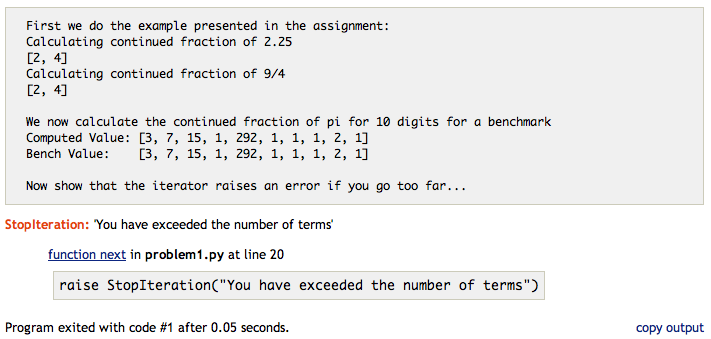
\includegraphics[height=3in]{include/prob1test.png}
    \caption{Output generated from test routine for Problem 1}
    \label{fig:include_prob1test}
\end{figure}\noindent
The results of Figure \ref{fig:include_prob1test} show that the continued fraction of $2.25 (9/4)$ is indeed $[2,4]$ as we are shown in the handout. Similarly, the script produces the correct result for the first 10 convergents of $\pi$.
The final requirement was that the script produce an exception if the user attempts to perform more iterations than there are coefficients. This is shown in Fig. \ref{fig:include_prob1test} by the exception \emph{StopIteration}.
% subsection results (end)
% section continued_fraction_representation_using_an_iterator (end)

%!TEX root = ../main.tex
% file: problem2.tex
\section{Stirling Numbers} % (fold)
\label{sec:stirling_numbers}
We wish to generate Stirling numbers of the first kind which are calculated using the recurrence
\begin{equation}
    \label{eq:stirling}
    c(n,k) = -(n-1)\times c(n-1,k) + c(n-1,k-1), \mbox{for } n \ge1 \mbox{ and } k \ge 1
\end{equation}
and the initial conditions $c(n,k)=0$ if $n\le0$ or $k\le0$, and $c(0,0)=1$. We intend to write a script which contains a class with the recursive function as well a dictionary which may be used to store previous values.

\subsection{Program Description} % (fold)
\label{sub:program_description2}
We begin by creating a class who's initializer contains a dictionary for previously stored values.
\begin{lstlisting}[caption={Initialization}, label=lst:init2,firstnumber=3]
    def __init__(self, n, k):
        self.dict = {(0,0):1} #start with the initial condition (saves an if statement)
        self.answer = self.c(n,k)
\end{lstlisting}\noindent
In Listing \ref{lst:init2} we populate the dictionary \emph{self.dict} with one of our initial conditions: $c(0,0)=1$. This is done to avoid an additional conditional statement in the main routine.
\begin{lstlisting}[caption={Main Logic for Stirling Number Generation}, label=lst:main2,firstnumber=8]
    def c(self, n, k):
         """Computes stirling numbers either recursively or by looking up in dictionary"""
         if (n,k) in self.dict.keys():
             return self.dict[(n,k)]
         elif n<=0 or k<=0:
             return 0
         else:
             ans = - (n-1)*self.c(n-1,k) + self.c(n-1,k-1)
             self.dict[(n,k)] = ans
             return ans
\end{lstlisting}\noindent
In \ref{lst:main2} we see that there is a conditional statement with three possible conditions. We first check if the solution is already available in our dictionary to prevent unnecessary recursion and calculation; the second check performed is whether we are at an initial condition $n\le0$ or $k\le0$. Finally, if it is not an initial condition and we do not have the value in our dictionary, we calculate the result of Eq. \ref{eq:stirling}.
% subsection program_description (end)

\subsection{Results} % (fold)
\label{sub:results2}
A quick test was initially performed on the code to see whether it was producing the correct result. We called the class with the values $n=5$ and $k=2$ with the following results:
\begin{figure}[H]
    \centering
        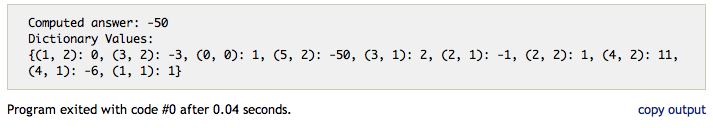
\includegraphics[width=6in]{include/prob2test.png}
    \caption{Testing of Program 2}
    \label{fig:include_prob2test}
\end{figure}
In Fig. \ref{fig:include_prob2test} we see the result $c(5,2)=-50$ which is the signed result. There was no specification of whether to produce signed or unsigned Stirling numbers, therefore they were left as signed. Similarly the dictionary is seen to have all necessary Stirling numbers from the recursion.



% subsection results (end)
% section stirling_numbers (end)

%!TEX root = ../main.tex
% file: problem2.tex
\section{Tkinter GUI for Adjacency Matrix} % (fold)
\label{sec:tkinter_gui_for_adjacency_matrix}
We wish to create a random adjacency matrix which carries the form
\begin{equation} \label{eq:A}
    A = \begin{pmatrix} 0 & B \\ B^T & 0 \end{pmatrix}.
\end{equation}
The coefficients $B$ are boolean integers representative of whether or not the index $i$ and $j$ are connected. We then wish to create a unit circle on a Tkinter canvas with vertices located at the coordinates $(cos(2k\pi/n),sin(2k\pi/n))$, where $k$ is the vertex number, and $n$ is the total number of vertices. After creation of the aforementioned unit circle and adjacency matrix, we connect the edges in Eq. \ref{eq:A} with lines on the canvas.

\subsection{Program Description} % (fold)
\label{sub:program_description3}
The script for Problem 3 is divided into two files. The first contains the reusable functions \emph{ranSymMatrix} and \emph{genVertList}. The second file contains the GUI specific operations. 

\begin{lstlisting}[caption={Generation of a Random Adjacency Matrix}, label=lst:ranSym,firstnumber=4]
    def ranSymMatrix(n):
        """Creates a symmetric random matrix """
        arr = numpy.random.random_integers(0,1,size=(n,n))
        for x in range(len(arr)):
            arr[x,x] = 0
        return (arr + arr.T)//2
\end{lstlisting}\noindent
In Listing \ref{lst:ranSym} we generate a random matrix of zeros and ones on line 6. We then set all trace elements to zero, and finally mirror the top of the matrix over the diagonal. We then have a random symmetric matrix with zero diagonals.

\begin{lstlisting}[caption={Main GUI Button Logic}, label=lst:mainGui,firstnumber=33]
    def mainLogic(self):
        """Main execution loop when button is pressed"""
        self.canvas.delete('all')
        n = int(self.nEntry.get())
        
        self.vert = vert = genVertList(n)
        self.drawPoints(vert)
        
        self.conMat = conMat = ranSymMatrix(n)
        self.calcConn(conMat)
\end{lstlisting}\noindent
Our main logic when the button pressed is shown in Listing \ref{lst:mainGui}. We begin by clearing the canvas to ensure no previous results are displayed. We then evaluate the string in the entry box and cast it to an integer. The function $genVertList$ generates $n$ vertices on a unit circle. These vertices are then drawn on the canvas using \emph{drawPoints}. The next step is to generate our adjacency matrix and pass it to the function \emph{calcConn}, which calculates which vertices are connected and draws a line between them.
% subsection program_description (end)


\subsection{Results} % (fold)
\label{sub:results3}
As a test we run the script and ensure the that proper vertices are connected with edges. We also print out the corresponding adjacency matrix to verify the connections.
\begin{figure}[H]
    \centering
        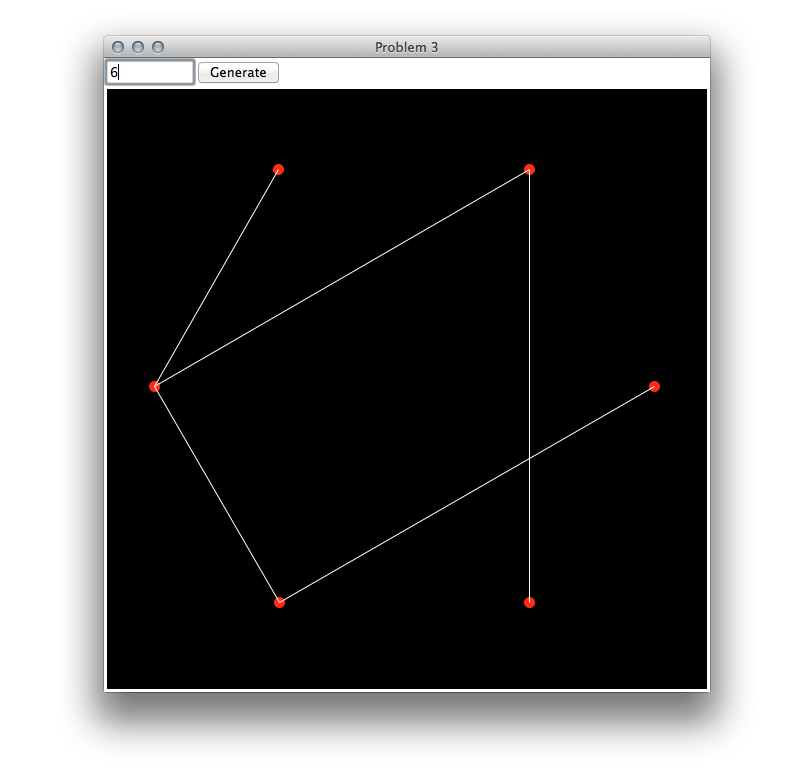
\includegraphics[width=6in,trim=1in 1in 1in 1in]{include/prob3gui.png}
    \caption{GUI for Problem 3}
    \label{fig:include_prob3gui}
\end{figure}
In Figure \ref{fig:include_prob3gui} we see that there are a total of 5 edges, which should be defined by the adjacency matrix
\begin{equation}\label{eq:adjM}
    A = 
    \begin{bmatrix}
        0 & 0 & 1 & 0 & 0 & 0 \\
        0 & 0 & 0 & 0 & 0 & 1 \\
        1 & 0 & 0 & 1 & 0 & 0 \\
        0 & 0 & 1 & 0 & 1 & 1 \\
        0 & 0 & 0 & 1 & 0 & 0 \\
        0 & 1 & 0 & 1 & 0 & 0 
    \end{bmatrix}
\end{equation}
We leave it as an exercise to the reader to verify that the adjacency matrix shown in Eq. \ref{eq:adjM} is represented in Figure \ref{fig:include_prob3gui}.
% subsection results (end)
% section tkinter_gui_for_adjacency_matrix (end)

%!TEX root = ../main.tex
% file: problem1.tex
\section{Animation of All Simple Paths of an Adjacency Matrix} % (fold)
\label{sec:animation_of_all_simple_paths_of_an_adjacency_matrix}

% section animation_of_all_simple_paths_of_an_adjacency_matrix (end)
\end{document}